\chapter{Fejlesztői dokumentáció} % Developer guide
\label{ch:impl}

\section{Tervezés}

\subsection{Probléma leírása}

\subsection{Felhasználói esetek}
\todo{Ez a kép nem felel meg a margónak, az baj? Legalább átlátható}
A felhasználói esetek a következőképpen néznek ki. A vállalkozó egyben felhasználó is, a felhasználók összes funkcióját tudják használni, ezt nem jelöltem a diagrammban, hogy átlátható maradjon.

\begin{figure}[H]
	\noindent\makebox[\textwidth]{
	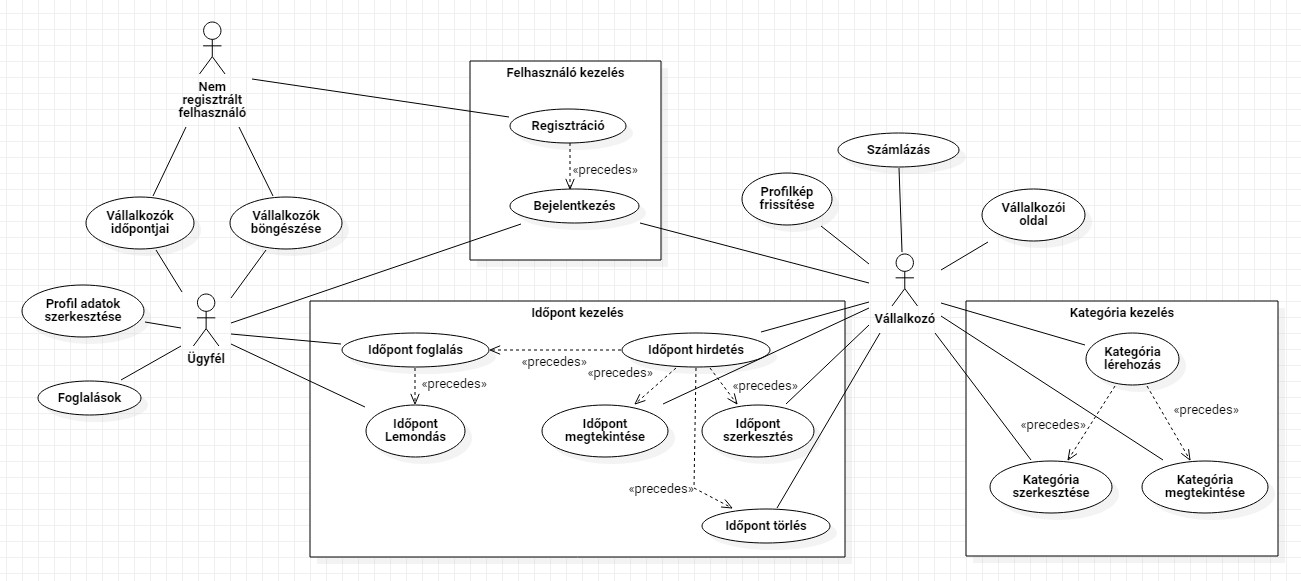
\includegraphics[width=1.3\textwidth]{usecase}}
	\caption{Felhasználói esetek}
	\label{fig:usecases}
\end{figure}

\begin{table}[H]
	\centering
	\begin{tabular}{|l|l|c|}
		\hline
		& \textbf{Leírás} & \textbf{Kód} \\
		\hline
		GIVEN & Nincs bejelentkezve & \multirow{3}{*}{asd} \\ \cline{1-2}
		WHEN & Bejelentkezéshez kötött oldalt nyitna meg & \\ \cline{1-2}
		THEN & Visszairányítódik a főoldalra & \\ 
		\hline
		GIVEN & asd & \multirow{3}{*}{asd} \\ \cline{1-2}
		WHEN & asd & \\ \cline{1-2}
		THEN & asd & \\ 
		\hline
		GIVEN & asd & \multirow{3}{*}{asd} \\ \cline{1-2}
		WHEN & asd & \\ \cline{1-2}
		THEN & asd & \\ 
		\hline
		GIVEN & asd & \multirow{3}{*}{asd} \\ \cline{1-2}
		WHEN & asd & \\ \cline{1-2}
		THEN & asd & \\ 
		\hline
		GIVEN & asd & \multirow{3}{*}{asd} \\ \cline{1-2}
		WHEN & asd & \\ \cline{1-2}
		THEN & asd & \\ 
		\hline
		GIVEN & asd & \multirow{3}{*}{asd} \\ \cline{1-2}
		WHEN & asd & \\ \cline{1-2}
		THEN & asd & \\ 
		\hline
		GIVEN & asd & \multirow{3}{*}{asd} \\ \cline{1-2}
		WHEN & asd & \\ \cline{1-2}
		THEN & asd & \\ 
		\hline
	\end{tabular}
\end{table}

\subsection{REST API vs MVC architektúra}
pro: frontnend és backend függetlensége, mobil appok, reaktivitás, skálázhatóság
contra: több kódbázis, integráció, api validáció

\subsection{Clean Architecture Backenden}
Clean architecture, UML diagrammok, dependency injection,
repo - controller - logika interakció

\subsection{Adatbázis - Entity Framework}
entity uml hivatkozások az előző részből

\subsection{Funkcionális Frontend}
React, react hooks, async result monád, reactive state changes


\section{Megvalósítás}
\subsection{Fejlesztési környezet}
Rider, vs code, visual studio, docker

dotnet, nuget

snowpack, node.js, yarn, react

???

\subsection{Fejlesztés közben felmerült problémák}
EF many-to-many, ef virtual classes nullable, sqlite inmemory test parallelization


\section{DevOps}
\subsection{CI/CD}
Github actions, cd dockerrel(?)
\subsection{Docker}
Dockerfile, dockerfile optimalizáció (alpine, builder, instruction layering - caching), docker compose

\section{Tesztelés}
\subsection{Unit tesztek}
Clean architecture, dependency injection, mockolás

\subsection{Integrációs tesztek}
httpclient, sqlite inmemory

\subsection{Manuális tesztek}
frontend tesztelés
























% Lorem ipsum dolor sit amet, consectetur adipiscing elit. Duis nibh leo, dapibus in elementum nec, aliquet id sem. Suspendisse potenti. Nullam sit amet consectetur nibh. Donec scelerisque varius turpis at tincidunt.


% \section{Tételek, definíciók, megjegyzések} % Theorem-like items

% \begin{definition}
% Mauris tristique sollicitudin ultrices. Etiam tristique quam sit amet metus dictum imperdiet. Nunc id lorem sed nisl pulvinar aliquet vitae quis arcu. Morbi iaculis eleifend porttitor.
% \end{definition}

% Maecenas rutrum eros sem, pharetra interdum nulla porttitor sit amet. In vitae viverra ante. Maecenas sit amet placerat orci, sed tincidunt velit. Vivamus mattis, enim vel suscipit elementum, quam odio venenatis elit, et mollis nulla nunc a risus. Praesent purus magna, tristique sed lacus sit amet, convallis malesuada magna. Phasellus faucibus varius purus, nec tristique enim porta vitae.

% \begin{theorem}
% Nulla finibus ante vel arcu tincidunt, ut consectetur ligula finibus. Mauris mollis lectus sed ipsum bibendum, ac ultrices erat dictum. Suspendisse faucibus euismod lacinia. Etiam vel odio ante.
% \end{theorem}
% \begin{proof}
% Etiam pulvinar nibh quis massa auctor congue. Pellentesque quis odio vitae sapien molestie vestibulum sit amet et quam. Pellentesque vel dui eget enim hendrerit finibus at sit amet libero. Quisque sollicitudin ultrices enim, nec porta magna imperdiet vitae. Cras condimentum nunc dui.
% \end{proof}

% Donec dapibus sodales ante, at scelerisque nunc laoreet sit amet. Mauris porttitor tincidunt neque, vel ullamcorper neque pulvinar et. Integer eu lorem euismod, faucibus lectus sed, accumsan felis. 

% \begin{remark}
% Nunc ornare mi at augue vulputate, eu venenatis magna mollis. Nunc sed posuere dui, et varius nulla. Sed mollis nibh augue, eget scelerisque eros ornare nec. Praesent porta, metus eget eleifend consequat, eros ligula eleifend ex, a pellentesque mi est vitae urna. Vivamus turpis nunc, iaculis non leo eget, mattis vulputate tellus.
% \end{remark}

% Fusce in aliquet neque, in pretium sem. Donec tincidunt tellus id lectus pretium fringilla. Nunc faucibus, erat pretium tempus tempor, tortor mi fringilla neque, ac congue ex dui vitae mauris. Donec pretium et quam a cursus.

% \begin{note}
% Aliquam vehicula luctus mi a pretium. Nulla quam neque, maximus nec velit in, aliquam mollis tortor. Aliquam erat volutpat. Curabitur vitae laoreet turpis. Integer id diam ligula.
% \end{note}

% Ut sollicitudin tempus urna et mollis. Aliquam et aliquam turpis, sed fermentum mauris. Nulla eget ex diam. Donec eget tellus pharetra, semper neque eget, rutrum diam.

% \subsection{Egyenletek, matematika} % Equations, formulas

% Duis suscipit ipsum nec urna blandit, $2 + 2 = 4$ pellentesque vehicula quam fringilla. Vivamus euismod, lectus sit amet euismod viverra, dolor metus consequat sapien, ut hendrerit nisl nulla id nisi. Nam in leo eu quam sollicitudin semper a quis velit.

% $$a^2 + b^2 = c^2$$

% Phasellus mollis, elit sed convallis feugiat, dolor quam dapibus nibh, suscipit consectetur lacus risus quis sem. Vivamus scelerisque porta odio, vitae euismod dolor accumsan ut.

% In mathematica, identitatem Euleri (equation est scriptor vti etiam notum) sit aequalitatem Equation~\ref{eq:euler}:
% \begin{equation}\label{eq:euler}
% e^{i \times \pi} + 1 = 0
% \end{equation}


% \section{Forráskódok} % Source code samples

% Nulla sodales purus id mi consequat, eu venenatis odio pharetra. Cras a arcu quam. Suspendisse augue risus, pulvinar a turpis et, commodo aliquet turpis. Nulla aliquam scelerisque mi eget pharetra. Mauris sed posuere elit, ac lobortis metus. Proin lacinia sit amet diam sed auctor. Nam viverra orci id sapien sollicitudin, a aliquam lacus suscipit. Quisque ac tincidunt leo Code~\ref{src:cpp} and \ref{src:csharp}:

% \lstset{caption={Hello World in C++}, label=src:cpp}
% \begin{lstlisting}[language={C++}]
% #include <stdio>

% int main() 
% {
% 	int c;
% 	std::cout << "Hello World!" << std::endl;

% 	std::cout << "Press any key to exit." << std::endl;
% 	std::cin >> c;
	
% 	return 0;
% }
% \end{lstlisting}

% \lstset{caption={Hello World in C\#}, label=src:csharp}
% \begin{lstlisting}[language={[Sharp]C}]
% using System;
% namespace HelloWorld
% {
% 	class Hello 
% 	{
% 		static void Main() 
% 		{
% 			Console.WriteLine("Hello World!");
			
% 			Console.WriteLine("Press any key to exit.");
% 			Console.ReadKey();
% 		}
% 	}
% }
% \end{lstlisting}

% \subsection{Algoritmusok} % Algorithms

% A general Interval Branch and Bound algorithm is shown in Algorithm~\ref{alg:ibb}. One of the following selection rules is applied in Step \ref{step:selrule}.\\
% Példa forrása: \href{https://www.inf.u-szeged.hu/actacybernetica/}{Acta Cybernetica (ez egy link)}.

% \begin{algorithm}[H]
% \caption{A general interval B\&B algorithm} 
% \label{alg:ibb} 
% \textbf{\underline{Funct}} IBB($S,f$)
% \begin{algorithmic}[1] % sorszámok megjelenítése minden n. sor előtt, most n = 1
% \STATE Set the working list ${\cal L}_W$ := $\{S\}$ and the final list ${\cal L}_Q$ := $\{\}$     
% \WHILE{( ${\cal L}_W \neq \emptyset$ )} \label{alg:igoend}
% 	\STATE  Select an interval $X$ from ${\cal L}_W$ \label{step:selrule}\COMMENT{Selection rule}  
% 	\STATE Compute $lbf(X)$ \COMMENT{Bounding rule}		  
% 	\IF[Elimination rule]{$X$ cannot be eliminated}
% 		\STATE Divide $X$ into $X^j,\ j=1,\dots, p$, subintervals   \COMMENT{Division rule}
% 		\FOR{$j=1,\ldots,p$}
% 			\IF[Termination rule]{$X^j$ satisfies the termination criterion}
% 				\STATE Store $X^j$ in ${\cal L}_W$ 
% 			\ELSE
% 				\STATE Store $X^j$ in ${\cal L}_W$ 
% 			\ENDIF
% 		\ENDFOR  
% 	\ENDIF
% \ENDWHILE
% \STATE \textbf{return} ${\cal L}_Q$
% \end{algorithmic}
% \end{algorithm}
